\chapter{Camera}
The camera in this game has a perspective view and always looks at the origin. The camera can be moved by using the W and S keys. The speed with which the camera can move may be altered using the T(slower) and R(faster) keys. Pressing Q puts the camera at the maximum angle and pressing E restores the camera view to normal (ie facing forwards). The parameters for this are found within \textbf{game.js} while the logic is found in the \textit{animate} function within \textbf{script.js}.

\begin{figure}[H]
	\centering
	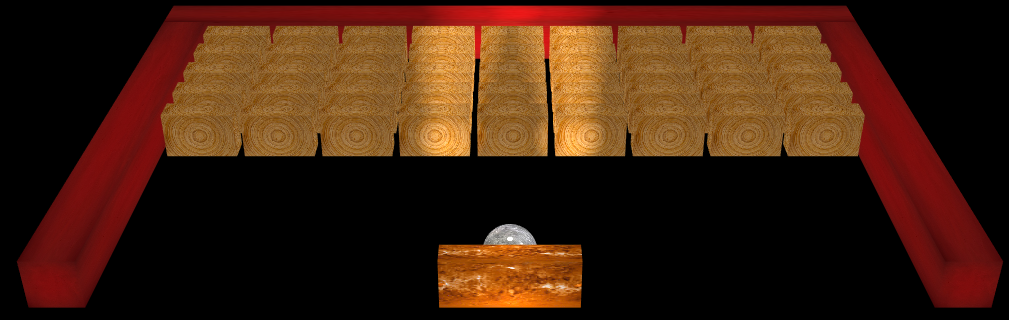
\includegraphics[width=\textwidth]{Images/Grazing.png}
	\caption{Camera looking a the scene at a grazing angle}
\end{figure}